This chapter aims to describe fundamental relationships between combinatorial optimization problems 
and linear programming. More specifically, we will define a new problem -- the vertex cover problem -- 
and show how this problem is intimately related to the matching problem through duality theory. 
We also use duality theory to shed light on the max-flow min-cut theorem.

\begin{section}{The Vertex Cover Problem}
	We begin this section by defining the vertex cover problem. 
	Again, this is a problem that can be 
	posed for graphs in general (not necessarily bipartite), but we will be restricting our 
	attention to bipartite graphs. 
	This is a good idea for many reasons, the most pertinent being that this problem is NP-
	complete in the general case.
	\begin{definition}
		Let $G = (U,V,E)$ be a bipartite graph. A subset $C\subset U\cup V$ is said to be a 
		\emph{vertex cover} if for each $(u,v)\in E$ we have that either $u\in C$ or $v\in C$. A 
		vertex cover $C$ on $G$ is a \emph{minimum vertex cover} if for any other vertex cover 
		$C\'$ on $G$, we have that $|C|\leq |C\'|$.
	\end{definition}
	Using what we have already learned, we now can specify at least one relation between matchings 
	and vertex covers: namely, the set of all vertices incident to at least one edge in any maximum 
	matching forms a vertex cover. Figure 2.1 shows some examples of vertex covers on the 
	graph we looked at in the previous chapter.

	\begin{figure}[h]
		\centering
		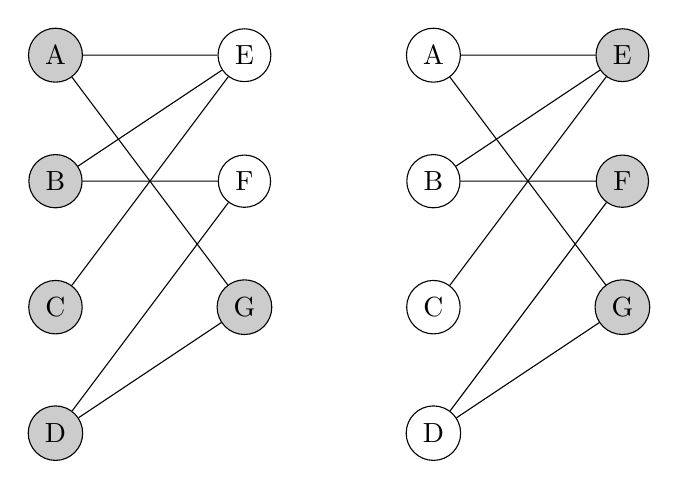
\begin{tikzpicture}[scale=.8,auto=left,every node/.style={circle,draw=black}]
		
		%left nodes
		\node[fill=black!20] (n1) at (1,10) {A};
		\node[fill=black!20] (n2) at (1,8) {B};
		\node[fill=black!20] (n3) at (1,6) {C};
		\node[fill=black!20] (n4) at (1,4) {D};

		%right nodes
		\node (n5) at (4,10) {E};
		\node (n6) at (4, 8) {F};
		\node[fill=black!20] (n7) at (4, 6) {G};
		
		%edges
		\draw (n1) -- (n5);
		\draw (n1) -- (n7);
		\draw (n2) -- (n5);
		\draw (n2) -- (n6);
		\draw (n3) -- (n5);
		\draw (n4) -- (n6);
		\draw (n4) -- (n7);

		%left nodes
		\node (m1) at (7,10) {A};
		\node (m2) at (7,8) {B};
		\node (m3) at (7,6) {C};
		\node (m4) at (7,4) {D};

		%right nodes
		\node[fill=black!20] (m5) at (10,10) {E};
		\node[fill=black!20] (m6) at (10, 8) {F};
		\node[fill=black!20] (m7) at (10, 6) {G};
		
		%edges
		\draw (m1) -- (m5);
		\draw (m1) -- (m7);
		\draw (m2) -- (m5);
		\draw (m2) -- (m6);
		\draw (m3) -- (m5);
		\draw (m4) -- (m6);
		\draw (m4) -- (m7);

		\end{tikzpicture}
		\caption{Examples of vertex covers.}
	\end{figure}
	You can convince yourself that the cover on the right is a minimum cover, i.e. there are no 
	vertex covers on this graph of size less than three. This brings will bring us 
	to an important theorem, but we must first prove a lemma.

	\begin{lemma}
		Let $G=(U,V,E)$ be a bipartite graph. Let $M$ be a matching on $G$ and $C$ a vertex 
		cover on $G$ such that $|M| = |C|$. Then $M$ is a maximum matching and $C$ is a minimum 
		vertex cover.
	\end{lemma}

	\begin{proof}
		Let $M\'$ be a maximum matching on $G$ and $C\'$ a be a minimum vertex cover on $G$. 
		For each $(u,v)\in M\'$, $C\'$ must include either $u$ or $v$, which tells us that 
		$|M\'| \leq |C\'|$. We then have  
		\[
			|M|\leq |M\'| \leq |C\'| \leq |C|.
		\]
		Thus, if $|M| = |C|$ we have equalities above, which means that the size of a maximum 
		matching is equal to the size of a minimum covering.
	\end{proof}
	Before we prove the following theorem, we want to be able to talk about collections of 
	alternating paths, as it will be useful to us in discussing the methods of finding maximum 
	matchings on graphs.
	\begin{definition}
		Let $G = (U,V,E)$ be a bipartite graph, and $M$ a matching on $G$. An 
		\emph{alternating tree} with respect to $M$ is a tree which satisfies two 
		conditions:
		\begin{itemize}
			\item the tree contains exactly one node $u\in U$. We call $u$ the 
				\emph{root} of the tree.
			\item all paths between the root and any other node in the tree are 
				alternating paths.
		\end{itemize}
	\end{definition}
	\begin{figure}[h]
		\centering
		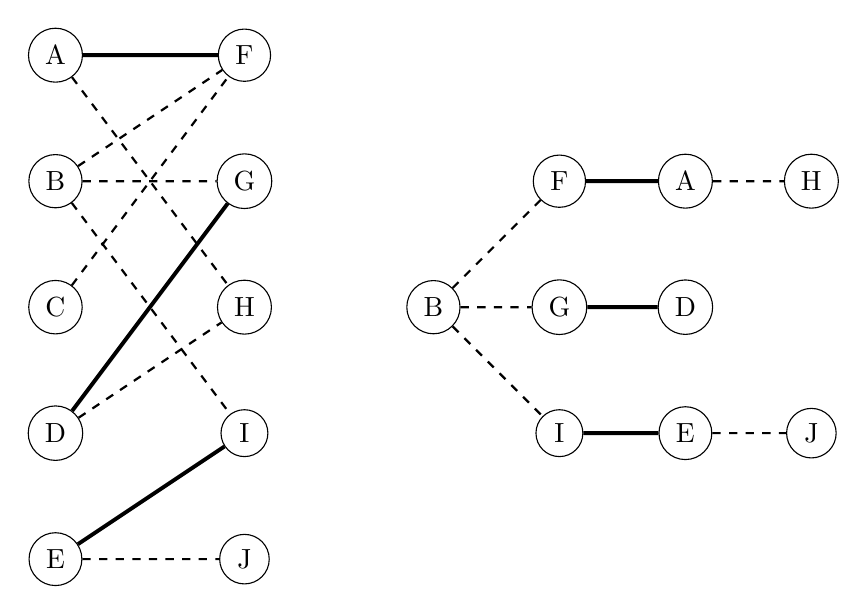
\begin{tikzpicture}[scale=.8,auto=left,every node/.style={circle,draw=black}]
		
		%left nodes
		\node (n1) at (1,10) {A};
		\node (n2) at (1,8) {B};
		\node (n3) at (1,6) {C};
		\node (n4) at (1,4) {D};
		\node (n5) at (1,2) {E};

		%right nodes
		\node (n6) at (4,10) {F};
		\node (n7) at (4,8) {G};
		\node (n8) at (4,6) {H};
		\node (n9) at (4,4) {I};
		\node (n10) at (4,2) {J};
		
		%edges
		\draw[line width=0.5mm] (n1) -- (n6);
		\draw[thick,dashed] (n1) -- (n8);
		\draw[thick,dashed] (n2) -- (n6);
		\draw[thick,dashed] (n2) -- (n7);
		\draw[thick,dashed] (n3) -- (n6);
		\draw[line width=0.5mm] (n4) -- (n7);
		\draw[thick,dashed] (n4) -- (n8);
		\draw[thick,dashed] (n2) -- (n9);
		\draw[line width=0.5mm] (n5) -- (n9);
		\draw[thick,dashed] (n5) -- (n10);

		%alternating tree
		\node (n11) at (7,6) {B};
		\node (n12) at (9,8) {F};
		\node (n13) at (9,6) {G};
		\node (n14) at (9,4) {I};
		\node (n15) at (11,8) {A};
		\node (n16) at (11,6) {D};
		\node (n17) at (11,4) {E};
		\node (n18) at (13,8) {H};
		\node (n20) at (13,4) {J};

		%tree edges
		\draw[thick,dashed] (n11) -- (n12);
		\draw[thick,dashed] (n11) -- (n13);
		\draw[thick,dashed] (n11) -- (n14);
		\draw[line width=0.5mm] (n12) -- (n15);
		\draw[line width=0.5mm] (n13) -- (n16);
		\draw[line width=0.5mm] (n14) -- (n17);
		\draw[thick,dashed] (n15) -- (n18);
		\draw[thick,dashed] (n17) -- (n20);
		\end{tikzpicture}
		\caption{Bipartite graph with matching (left) and corresponding alternating tree 
		rooted at vertex B (right).}
	\end{figure}

	\begin{theorem}{(K\H{o}nig-Egervary)}
		For any bipartite graph $G$, if $M$ is a maximum matching on $G$ and $C$ is a minimum 
		vertex cover  on $G$, then $|M| = |C|$.
	\end{theorem}
	\begin{proof}
		Let $G=(U,V,E)$ be a bipartite graph, and let $M$ be a maximum matching on $G$. 
		Furthermore, define
		\begin{align}
			F &:= \{u\in U\; |\; u \text{ unmatched}\}\\
			R &:= \{\text{all vertices connected to vertices in $F$ by alternating paths}\}.
		\end{align}
		Let $S = R\cap U$ and $T = R\cap V$. Denote $N(S)$ to be the set of all vertices 
		connected to elements of $S$ (i.e. the ``neighbors'' of $S$). Then we have the following:
		\begin{align*}
			&(1)\text{ Every vertex in $T$ is matched;}\\
			&(2)\ N(S) = T.
		\end{align*}
		The first claim comes from the fact that, if $M$ is a 
		maximum matching, then our alternating paths that start at a vertex in $F$ must have 
		an even length $\geq 2$. Otherwise, we would have an augmenting path, 
		which contradicts our assumption that $M$ is a maximum matching.
		The second claim comes from the fact that every node in $N(S)$ is connected to vertices 
		in $F$ by an alternating path. 

		Now, define $C := (U\setminus S)\cup T$. Every edge 
		in $G$ must have one of its endpoints in $C$. If not, then there would be an 
		edge with one endpoint in $S$ and one endpoint in $V\setminus T$, which contradicts 
		$N(S) = T$. Therefore $C$ is a vertex cover of $G$. Moreover, $|C| = |M|$, since for each 
		edge in $M$ we've included one of its endpoints in $C$ (the vertices we've chosen are 
		those in $N(S)$ and those in $U\setminus S$). Thus, by the previous lemma, $C$ is 
		a minimum covering.
	\end{proof}

	This theorem and lemma tell us that there is a deep relationship between maximum matchings and 
	minimum vertex covers on bipartite graphs. Subsequently, given a solution to a maximum matching 
	problem, we can turn it into a solution to a minimum vertex cover problem, and vice versa. Our 
	goal now is to generalize this concept.
\end{section}

\begin{section}{Duality Theory}
	We now turn to duality theory, which allows us to speak more generally about the relationships 
	between certain combinatorial problems that we are interested in solving.
	\begin{definition}
		Let the \emph{primal linear program} be the following linear program.
		\begin{alignat}{3}
			& \text{maximize } & \sum_{i=1}^{n} c_{i} x_{i}& \\
			& \text{subject to } \quad & \sum_{i=1}^{n} a_{ij} x_{i} & \leq b_{j}, & j & 
			= 1, \dots , m \\
					&& x_{i} & \geq 0, \quad & i & = 1, \dots, n.
		\end{alignat}		
		Then we define the \emph{dual linear program} of this primal linear program to be the 
		following linear program.
		\begin{alignat}{3}
			& \text{minimize } & \sum_{j=1}^{m} b_{j} y_{j}& \\
			& \text{subject to } \quad & \sum_{j=1}^{n} a_{ij} y_{j} & \geq c_{i}, & i & 
			= 1, \dots , m \\
					&& y_{j} & \geq 0, \quad & j & = 1, \dots, n.
		\end{alignat}		

		The dual of the dual is always the primal.
	\end{definition}
	In some settings we instead 
	have a minimization problem (the dual here) acting as the primal problem, while the maximization 
	problem is actually the dual. Ultimately, it does not matter which one we call the dual and
	which one we call the primal; what matters is how they relate to each other. 
	Let us introduce some 
	notation. First, let us denote the primal maximization problem by $\Gamma$, and 
	the dual minimization problem by $\Omega$. For a given linear program, we denote 
	an optimal solution by $\mathbf{OPT}$, by which we mean the value that optimizes the objective 
	function and satisfies the linear constraints. Naturally, we want to know how solutions to 
	linear programs that are primal-dual to each other relate.

	\begin{theorem}{(Weak duality)}
		If the primal linear program (in maximization form) and the dual (in minimization 
		form) are both feasible, then 
		\[
			\mathbf{OPT}(\Gamma) \leq \mathbf{OPT}(\Omega).
		\]
	\end{theorem}

	\begin{proof}
		Suppose that $\mathbf{x} = (x_1, x_2,\dots,x_n)$ is a feasible solution to $\Gamma$, and 
		$\mathbf{y} = (y_1, y_2, \dots y_m)$ is a feasible solution to $\Omega$. 
		So $\mathbf{OPT}(\Gamma) = \sum_{i=1}^{n} c_i x_i$ and 
		$\mathbf{OPT}(\Omega) = \sum_{j=1}^{n} b_j y_j$.
		Because 
		$\mathbf{y}$ is dual feasible and all $x_i$ and $y_j$ are nonnegative, we have 
		\[
			\sum_{j=1}^{m} b_j y_j \geq \sum_{j=1}^{m}\left(\sum_{i=1}^{n} a_{ij}x_i\right) 
			y_j.
		\]
		Similarly, we have that 
		\[
			\sum_{i=1}^{n} c_i x_i \leq \sum_{i=1}^{n}\left(\sum_{j=1}^{m} a_{ij} y_j\right) 
			x_i.
		\]
		Note that by rearranging terms, we have the following equality:
		\[
			\sum_{i=1}^{n}\left(\sum_{j=1}^{m} a_{ij} y_j\right) 
			x_i =
			\sum_{j=1}^{m}\left(\sum_{i=1}^{n} a_{ij}x_i\right) 
			y_j,
		\]
		which shows that 
		\[
			\sum_{i=1}^{n} c_i x_i \leq 
			\sum_{i=1}^{n}\left(\sum_{j=1}^{m} a_{ij} y_j\right) 
			x_i =
			\sum_{j=1}^{m}\left(\sum_{i=1}^{n} a_{ij}x_i\right) 
			y_j \leq 
			\sum_{j=1}^{m} b_j y_j,
		\]
		so $\mathbf{OPT}(\Gamma) \leq \mathbf{OPT}(\Omega)$.
	\end{proof}
	What's surprising is the following theorem.

	\begin{theorem}{(Strong duality)}
		Given two linear programs $\Gamma$ and $\Omega$ that are duals of each other, if one is 
		feasible and bounded, then so is the other. Additionally, 
		\[
			\mathbf{OPT}(\Gamma) = \mathbf{OPT}(\Omega).
		\]
	\end{theorem} 
	In Chapter 4 we will use duality theory to get necessary and sufficient conditions for 
	$\mathbf{OPT}(\Gamma) = \mathbf{OPT}(\Omega)$, which will give us \textbf{Theorem 2.6}.
	Our goal now is to use facts about duality to better understand the relationships between 
	our combinatorial optimization problems.

\begin{subsection}{Maximum-Matching Duality}
	Let us formulate the maximum matching as a linear program. Our goal is to maximize the number 
	of edges in our matching. Let us define a set of variables $x_{uv}$, one for each $(u,v)\in E$. 
	These will be the unknowns in the linear program. We will use these to define a subset of 
	edges as follows: when $x_{uv} = 1$, we will say that $(u,v)$ is included in that subset; 
	when $x_{uv} = 0$, we will say that $(u,v)$ is excluded from that subset. Since we are trying 
	to construct a matching on our graph, we need the constraints that ensure no edge is incident to 
	more than one vertex in the matching; otherwise, the matching would be invalid. For a fixed 
	vertex $u\in U$, the number of edges in the matching incident 
	to $u$ is given by $\sum_{v\in V} x_{uv}$. So we want this to be less than or equal to one. 
	Similarly, for any vertex $v\in V$, we want $\sum_{u\in U} x_{uv}$ to be less than or equal to 
	one. This gives us the following linear program:
	\begin{alignat}{3}
		& \text{maximize } & \sum_{u,v} x_{uv}& \\
		& \text{subject to } \quad & \sum_{v} x_{uv} & \leq 1, & \quad \text{for all } u\in U& \\
				     &\quad & \sum_{u} x_{uv} & \leq 1, & \quad \text{for all } v\in 
				     V & \\
				&& x_{uv} & \in \{0,1\}.
	\end{alignat}

	What we have presented here is an $\emph{integer}$ linear program, since we've restricted our 
	$x$ variables to be integers. In general, solving integer linear programs is NP-hard. However, 
	in this case it is well known that this linear program attains an integer solution at extreme 
	points
	(see Birkhoff \cite{birkhoff1946} and von Neumann \cite{vN53})
	of the polyhedron solution space, so we can drop the integrality requirements and just say 
	$x_{uv} \geq 0$.

	Now let us try and construct the dual of this linear program. To do this we will need a variable 
	$y_u$ for each vertex $u$. Similarly, we need a variable $y_v$ for each vertex $v$. Our 
	objective will be to minimize over the sum of these $y_u$ and $y_v$. Since our coefficient on 
	$x_{uv}$
	in the primal is the constant vector one, our only constraint will be that $y_u + y_v \geq 1$. 
	This gives us the dual linear program:
	\begin{alignat}{3}
		& \text{minimize } & \sum_{u\in U} y_u + \sum_{v\in V} y_v& \\
		& \text{subject to } \quad & y_u + y_v & \geq 1, & \quad \text{for all } 
					(u,v)\in E & \\
				    && y_u,y_v & \geq 0.
	\end{alignat}
	This dual problem tells us that each edge must be ``covered'' by at least one of its incident 
	vertices. This is exactly the vertex cover problem! So, for unweighted bipartite graphs, the 
	linear programs for maximum matchings and minimum vertex covers are duals of each other. 
	We will use this insight to construct our algorithms for solving the maximum matching problem. 

	There is another variant of the maximum matching problem called the 
	\emph{maximum weight matching problem}. In this 
	version, we are given a bipartite graph with non-negative edge weights $w_{uv}$ for all 
	edges $(u,v)\in E$. Instead of trying to maximize the number of edges in the matching, the goal 
	is to find a matching $M$ such that $\sum_{(u,v) \in M} w_{uv}$, or the total ``weight'' of the 
	matching, is greater than the weight of any other matching. 
	We can easily encode this problem by making 
	a slight modification to our linear program from before. The primal is given by the following 
	linear program:
	\begin{alignat}{3}
		& \text{maximize } & \sum_{u,v} w_{uv}x_{uv}& \\
		& \text{subject to } \quad & \sum_{v} x_{uv} & \leq 1, & \quad 
					\text{for all } u\in U& \\
				     &\quad & \sum_{u} x_{uv} & \leq 1, & \quad 
				     	\text{for all } v\in V & \\
				&& x_{uv} & \geq 0.
	\end{alignat}
	Then the dual is given by:
	\begin{alignat}{3}
		& \text{minimize } & \sum_{u} y_u + \sum_v y_v& \\
		& \text{subject to } \quad & y_u + y_v & \geq w_{uv}, & \quad \text{for all } 
					(u,v)\in E & \\
				    && y_u,y_v & \geq 0.
	\end{alignat}
	The dual is a sort of weighted vertex cover. One way to think about it is that each edge 
	has a ``cost'' given by $w_{uv}$, and each of its endpoints (vertices) must pool ``money'' 
	in order 
	to pay at least that cost. So instead of edges being covered or not covered, there is a certain 
	``amount'' that they have to be covered.

	These two problems, the maximum weight matching and the minimum weight vertex cover, are the 
	problems that the Hungarian algorithm solves, which we discuss in Chapter 3. For now, we digress 
	and discuss the max-flow min-cut theorem, as an ode to students who have taken a course in 
	algorithms.
\end{subsection}

\begin{subsection}{The Max-Flow Min-Cut Theorem}
	Here we demonstrate that a common problem discussed in algorithms courses, and a quite 
	amazing theorem, is really a special case of what we have been discussing. 
	We first recall the definition of a flow network.
	\begin{definition}
		A \emph{flow network} $G = (V,E)$ is a directed graph in which each edge $(u,v)\in E$ 
		has an assigned \emph{capacity} $c_{uv} \geq 0$. Furthermore, there are two 
		distinguished vertices in $V$, a source $s$ and a sink $t$. 
		We assume that every $v\in V$ lies in some path $s\to \cdots \to v\to \cdots \to t$.
	\end{definition}
	Given a flow network, we can define a function on the network.
	\begin{definition}
		Let $G = (V,E)$ be a flow network. A \emph{flow} on $G$ is a function $f: V\times V \to 
		\R$ that satisfies the following:
		\begin{itemize}
			\item Capacity constraint: For all $u,v\in V$, $0\leq f(u,v) \leq 
				c_{uv}$.
			\item Flow conservation: For all $u\in V\setminus \{s,t\}$, we have 
				\[
					\sum _{v\in V} f(v,u) = \sum_{v\in V} f(u,v).
				\]
				This says that, for all vertices $v$ except our source and sink, the 
				flow out of $v$ is equal to the flow into $v$. 
		\end{itemize}
		We define the value of the flow to be $val(f) = \sum_{v\in V} f(s,v) - \sum_{v\in V} 
		f(v,s)$, which is just the flow out of our source minus the flow into our source.
	\end{definition}
	\begin{figure}[h]
		\centering
		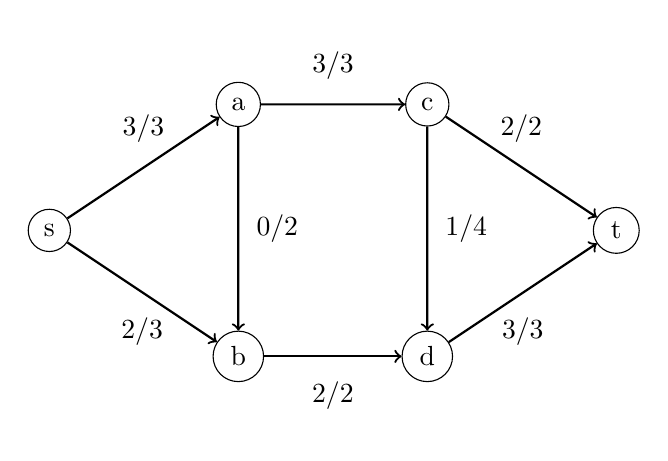
\begin{tikzpicture}[scale=.8,auto=left,every node/.style={circle,draw=black}]
			\node (n1) at (3,3) {s};
			\node (n2) at (6,5) {a};
			\node (n3) at (6,1) {b};
			\node (n4) at (9,5) {c};
			\node (n5) at (9,1) {d};
			\node (n6) at (12,3) {t};

			\draw[->,thick] (n1) -- node[draw=none, above] {3/3} ++ (n2);
			\draw[->,thick] (n1) -- node[draw=none, below] {2/3} ++ (n3);
			\draw[->,thick] (n2) -- node[draw=none, right] {0/2} ++ (n3);
			\draw[->,thick] (n2) -- node[draw=none, above] {3/3} ++ (n4);
			\draw[->,thick] (n3) -- node[draw=none, below] {2/2} ++ (n5);
			\draw[->,thick] (n4) -- node[draw=none, right] {1/4} ++ (n5);
			\draw[->,thick] (n4) -- node[draw=none, above] {2/2} ++ (n6);
			\draw[->,thick] (n5) -- node[draw=none, below] {3/3} ++ (n6);
		\end{tikzpicture}
		\caption{Flow network with maximum flow of 5. Notation: $X/Y$ means an edge has capacity 
		$Y$ and flow $X$, given by the flow function.}
	\end{figure}
	In Figure 2.3, (from Cormen, Leiserson, Rivest, and Stein \cite{cormen2009introduction}) 
	we have a flow network with a corresponding flow. For example, the capacity 
	of the edge $(s,b)$ is $3$, and our flow function in sending a flow of value $2$ through 
	this edge.

	The problem, as demonstrated in a typical algorithms course, is to find a maximum flow from $s$ 
	to $t$. This is done using a method developed by Ford and Fulkerson which looks for augmenting 
	paths in the residual graph (essentially the subgraph where the flows $f(u,v) < c_{uv}$. 
	The reader should refer to Cormen, Leiserson, Rivest, and Stein 
	\cite{cormen2009introduction} for a more detailed treatment. Now, we recall the definition 
	of a cut in a flow network.
	\begin{definition}
		An $s-t$ \emph{cut} $(S,T)$ of a flow network $G=(V,E)$ is a partition of $V$ into 
		sets $S$ and $T = V\setminus S$ such that $s\in S$ and $t\in T$. Given a flow $f$, the 
		\emph{net flow} $f(S,T)$ across the cut $(S,T)$ is defined as 
		\[
			f(S,T) = \sum_{u\in S} \sum_{v\in T} f(u,v) - \sum_{u\in S} \sum_{v\in T} 
			f(v,u).
		\]
		Finally, the \emph{capacity} of the cut is defined as $c(S,T) = 
		\sum_{u\in S} \sum_{v\in T} c(u,v)$. A \emph{minimum cut} has capacity less than or 
		equal to all other cuts in the network.
	\end{definition}
	One of the coolest and most surpising theorems in an algorithms course is that, given a flow 
	network $G$, the value of the maximum flow on $G$ is equal to the capacity of the minimum 
	$s-t$ cut of $G$.

	Our goal now is to build up to this same theorem using the tools developed in this chapter,
	following the treatment given by Vazirani \cite{vazirani2002approximation}. 
	We will first give a linear program for the 
	maximum flow problem. To make things simpler, let us introduce an arc of infinite capacity 
	from the sink $t$ to the source $s$; this converts this to a \emph{circulation} problem, 
	with the objective to maximize the flow $f(t,s)$. This allows us to enforce flow conservation 
	at $s$ and $t$ as well, which makes the corresponding linear program simpler. The linear 
	program is as follows:
	\begin{alignat}{3}
		& \text{maximize } & f(t,s)\\
		& \text{subject to } & f(u,v) &\leq c_{uv}, &\quad (u,v)\in E\\ 
				     && \sum_{v:(v,u)\in E} f(v,u) & \leq \sum_{v:(u,v)\in E} f(u,v), &
				     	\quad u\in V &\\
				     && f(u,v) &\geq 0. &\quad (u,v)\in E &
	\end{alignat}
	It is not immediately obvious why the second set of inequalities implies flow conservation; 
	at first glance all 
	it seems to say is that for each $u$, the total flow into $u$ is at most the total flow out 
	of $u$. However, note that if this holds for all $u$, we in fact have equality of incoming and 
	outgoing flow, since a deficit of flow at some $u$ implies a flow surplus at some $v$. So 
	this does in fact give us conservation of flow. 
	
	Now we want to find the dual of this program. 
	Our sense (hopefully) is that the dual will somehow relate to minimum cuts, given the 
	foreshadowing of the previous section. Let's see! We introduce variables $d_{uv}$ and $p_u$ for 
	inequalities (2.24) and (2.25), respectively. Then the dual linear program is as follows:
	\begin{alignat*}{3}
		& \text{minimize } & \sum_{(u,v)\in E} c_{uv} d_{uv}& \\
		& \text{subject to } \quad & d_{uv} - p_u + p_v & \geq 0, & \quad (u,v)\in E & \\
				    && p_s - p_t & \geq 1, & \\
				    && d_{uv} & \geq 0, & \quad (u,v) \in E & \\
				    && p_u,\ p_v & \geq 0.
	\end{alignat*}
	It is known that extreme point solutions to these linear programs take on values zero or one at 
	each coordinate. Let us now consider an optimal dual solution $(\mathbf{d}^{*},\mathbf{p}^{*})$. 
	First, in order to satisfy $p_s^{*} - p_{t}^{*} \geq 1$ with zero/one values, it must 
	be the case that $p_s^{*} = 1$ and $p_t^{*} = 0$. This motivates an $s-t$ cut $(S,T)$ 
	with $S$ consisting 
	of vertices with value one, and $T$ the vertices with value zero. For an edge $(u,v)$ such that 
	$u\in S$ and $v\in T$, we have that $p_u^{*} = 1$ and $p_v^{*} = 0$, so by the first constraint 
	$d_{uv}^{*} = 1$. This means that for any edge $(u,v)$ in the cut, the corresponding 
	$d_{uv}^{*} = 1$. Note that any other $d_{uv}^{*}$ where $(u,v)$ is not in the cut can take value 
	zero without violating the constraints (in fact we want these $d_{uv}^{*}=0$ since we are 
	minimizing our objective function). Thus the objective function's value is equal to the capacity 
	of this $s-t$ cut, which must be a minimum cut. Strong duality tells us that this corresponds 
	to the value of $f(t,s)$ in the primal linear program. 
	
	To make this clear, let us look back at our flow network in Figure 2.3. 
	We expect that, given our discussion of the dual, we should be able to find a cut 
	$(S,T)$ of the flow network that has value five. 
	Moreover, this cut $(S,T)$ should be such that $S$ consists of vertices with value one, 
	and $T$ consists of vertices with value zero. 
	We know that we must set $p_s = 1$ and $p_t = 0$. This gives us the following dual solution, 
	where grey vertices are in $S$ and white vertices are in $T$:
	\begin{figure}[H]
		\centering
		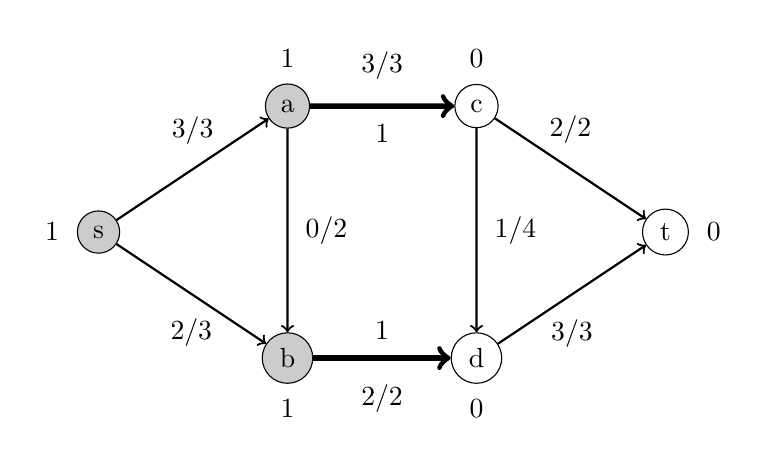
\begin{tikzpicture}[scale=.8,auto=left,every node/.style={circle,draw=black}]
			\node [fill=black!20, label=left:{1}] (n1) at (3,3) {s};
			\node [fill=black!20, label=above:{1}] (n2) at (6,5) {a};
			\node [fill=black!20, label=below:{1}] (n3) at (6,1) {b};
			\node [label=above:{0}] (n4) at (9,5) {c};
			\node [label=below:{0}] (n5) at (9,1) {d};
			\node [label=right:{0}] (n6) at (12,3) {t};

			\draw[->,thick] (n1) -- node[draw=none, above] {3/3} ++ (n2);
			\draw[->,thick] (n1) -- node[draw=none, below] {2/3} ++ (n3);
			\draw[->,thick] (n2) -- node[draw=none, right] {0/2} ++ (n3);
			\draw[->,line width=0.7mm] (n2) -- node[draw=none, above] {3/3} 
			node[draw=none, below] {1} ++ (n4);
			\draw[->,line width=0.7mm] (n3) -- node[draw=none, below] {2/2} 
			node[draw=none, above] {1} ++ (n5);
			\draw[->,thick] (n4) -- node[draw=none, right] {1/4} ++ (n5);
			\draw[->,thick] (n4) -- node[draw=none, above] {2/2} ++ (n6);
			\draw[->,thick] (n5) -- node[draw=none, below] {3/3} ++ (n6);
		\end{tikzpicture}
		\caption{Flow network with corresponding dual solution (bold edges are the edges in our 
		cut).}
	\end{figure}
	In Figure 2.4, the $s-t$ cut corresponds to the sets $S= \{\mbox{s},\mbox{a},\mbox{b}\}$ and 
	$T = \{\mbox{c},\mbox{d},\mbox{t}\}$; the 
	edges in the cut are the bold edges $(\mbox{a},\mbox{c})$ and $(\mbox{b},\mbox{d})$. 
	So the capacity of the cut is five, 
	which is what we'd expect. In order to make the figure readable, we leave out our dual labeling 
	on edges that are not in the cut (their label is ``0'' anyways). Edges in the cut have label 
	``1'', as shown in the figure. Note that our dual labeling of edges and vertices in this flow 
	network satisfies our dual constraints.

	Thus, we have given an alternative formulation of the max-flow min-cut relationship using 
	linear programs. In the next chapter, we present the main algorithm of this thesis, the 
	Hungarian algorithm, which is interesting in and of itself, and also as a tool to motivate 
	general primal-dual algorithms.
\end{subsection}
\end{section}
